\label{ap:serpent_gsrc}
% Serpent _gsrc format

This section presents an example of a \textit{\_gsrc.m} file produced by Serpent.
The output file is divided into materials and their respective nuclides.
For this work, the following columns contain the most valuable information.
First column is the ZAI of the nuclide, third column is the total gamma emission rate of the nuclide, fifth column is the gamma emission energy, and seventh column is the emission rate cumulative fraction for the gamma emission energy specified in the fifth column.
Figure \ref{fig:example_gsrc} displays the gamma source distribution for each nuclide specified in this example.

\begin{lstlisting}
mat_m1 = [

% --- Te-132 :

521320 1.84967E+00 1.27871E+16 4.11726E-01 2.28160E-01 8.80000E-01 4.75762E-01
521320 1.84967E+00 1.27871E+16 4.11726E-01 2.86120E-02 3.77008E-01 6.79586E-01
521320 1.84967E+00 1.27871E+16 4.11726E-01 2.83170E-02 2.04754E-01 7.90284E-01
521320 1.84967E+00 1.27871E+16 4.11726E-01 4.97200E-02 1.49600E-01 8.71164E-01
521320 1.84967E+00 1.27871E+16 4.11726E-01 3.94000E-03 7.83222E-02 9.13508E-01
521320 1.84967E+00 1.27871E+16 4.11726E-01 3.22950E-02 6.77639E-02 9.50144E-01
521320 1.84967E+00 1.27871E+16 4.11726E-01 3.22390E-02 3.51007E-02 9.69120E-01
521320 1.84967E+00 1.27871E+16 4.11726E-01 3.30470E-02 2.00692E-02 9.79970E-01
521320 1.84967E+00 1.27871E+16 4.11726E-01 1.16300E-01 1.96240E-02 9.90580E-01
521320 1.84967E+00 1.27871E+16 4.11726E-01 1.11760E-01 1.74240E-02 1.00000E+00

% --- Sr-92 :

380920 1.03234E+00 9.11055E+15 6.39262E-01 1.38393E+00 9.00000E-01 8.71809E-01
380920 1.03234E+00 9.11055E+15 6.39262E-01 9.53310E-01 3.51900E-02 9.05897E-01
380920 1.03234E+00 9.11055E+15 6.39262E-01 4.30490E-01 3.27600E-02 9.37631E-01
380920 1.03234E+00 9.11055E+15 6.39262E-01 2.41560E-01 2.92500E-02 9.65965E-01
380920 1.03234E+00 9.11055E+15 6.39262E-01 1.14235E+00 2.79000E-02 9.92991E-01
380920 1.03234E+00 9.11055E+15 6.39262E-01 6.50800E-01 3.69000E-03 9.96565E-01
380920 1.03234E+00 9.11055E+15 6.39262E-01 4.91270E-01 2.74500E-03 9.99224E-01
380920 1.03234E+00 9.11055E+15 6.39262E-01 8.92680E-01 8.01000E-04 1.00000E+00

% --- Zr-95 :

400950 9.91185E-01 4.03323E+15 8.43173E-01 7.56725E-01 5.43800E-01 5.48636E-01
400950 9.91185E-01 4.03323E+15 8.43173E-01 7.24192E-01 4.42700E-01 9.95273E-01
400950 9.91185E-01 4.03323E+15 8.43173E-01 1.65210E-02 4.37482E-03 9.99687E-01
400950 9.91185E-01 4.03323E+15 8.43173E-01 2.17000E-03 3.10473E-04 1.00000E+00

% --- Pd-112 :

461120 3.07251E-01 4.66930E+13 9.98279E-01 1.85000E-02 2.72000E-01 8.85268E-01
461120 3.07251E-01 4.66930E+13 9.98279E-01 2.98000E-03 3.52514E-02 1.00000E+00

% --- Ra-225 :

882250 4.36388E-01 4.94167E-01 1.00000E+00 4.00000E-02 3.00000E-01 6.87461E-01
882250 4.36388E-01 4.94167E-01 1.00000E+00 1.27000E-02 1.36388E-01 1.00000E+00
];
\end{lstlisting}

\begin{figure}[htbp!] %htbp! or H
  \centering
  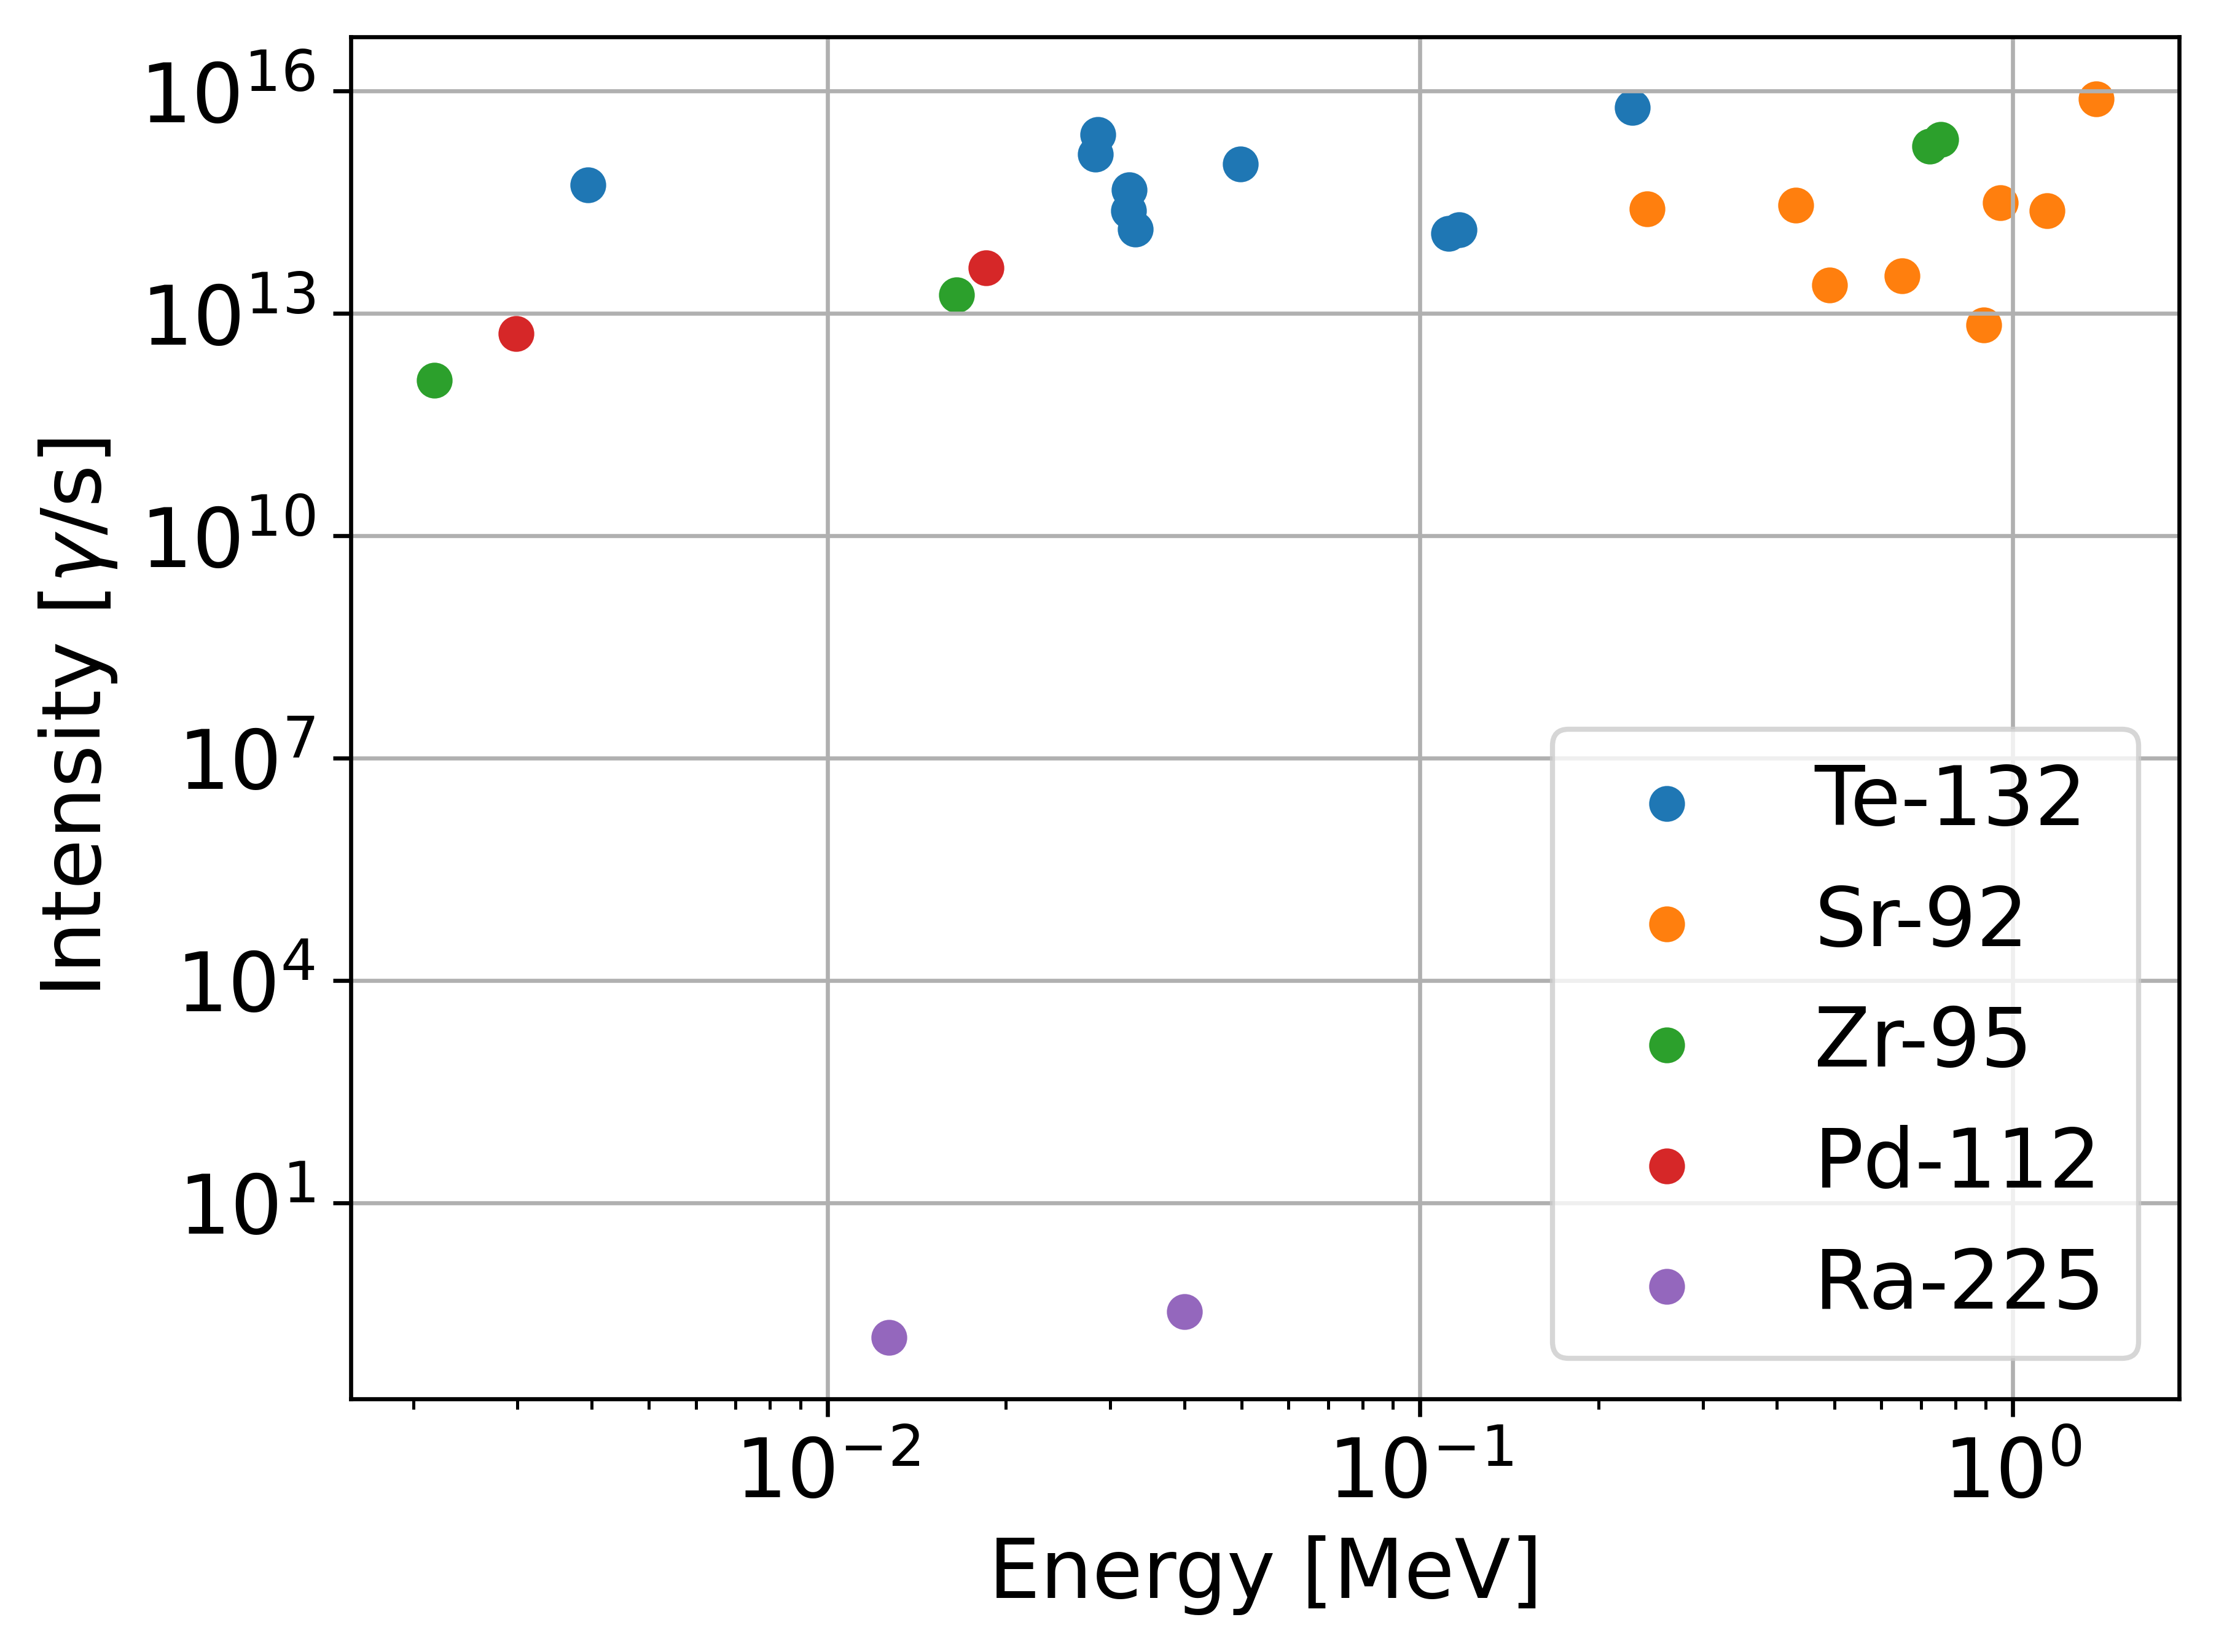
\includegraphics[width=0.75\linewidth]{figures/example_gsrc}
  \caption{Example of gamma source distribution produced by Serpent.}
  \label{fig:example_gsrc}
\end{figure}
